\documentclass[12pt,a4paper]{report}
\usepackage{titlesec}
\titleformat{\chapter}[display]{\bfseries\Huge}{{Chapter} \thechaptertitlename\thechapter}{0pt}{\Huge}[{\titlerule[1.5]}]
\titlespacing*{\chapter}{0pt}{0pt}{20pt}

\usepackage[top=0.70in, bottom=0.80in, left=0.8in,right=0.80in]{geometry}
\usepackage[pdftex]{graphicx}
\usepackage[bookmarks, colorlinks=false]{hyperref}
\hypersetup{pdfborder = {0 0 0}}

\usepackage[final]{pdfpages}
\usepackage{float}
\usepackage{hyperref}
\usepackage{pslatex}
\usepackage{array}
\usepackage{setspace}
\usepackage{enumerate}
\usepackage{longtable}
\usepackage{lipsum}
\usepackage[font=small,labelfont=bf]{caption}
\def\figurename{\textbf{Figure }}

\usepackage{listings}
\usepackage{color}
\definecolor{dkgreen}{rgb}{0,0.6,0}
\definecolor{gray}{rgb}{0.5,0.5,0.5}
\definecolor{mauve}{rgb}{0.58,0,0.82}
\lstset{
  language=Java,
  basicstyle=\footnotesize,
  numbers=left,
  numberstyle=\tiny\color{gray},
  stepnumber=1,
  numbersep=5pt,
  backgroundcolor=\color{white},
  showspaces=false,
  showstringspaces=false,
  showtabs=false,
  frame=single,
  rulecolor=\color{black},
  tabsize=2,
  captionpos=b,
  breaklines=true,
  breakatwhitespace=false,
  keywordstyle=\color{blue},
  commentstyle=\color{dkgreen},
  stringstyle=\color{mauve},
  escapeinside={\%*}{*)},
  morekeywords={*,...}
}

\usepackage{fancyhdr}
\fancypagestyle{plain}{%
\fancyfoot[L]{\emph{Department of Computer Science and Engineering(AI), SKIT, Jaipur}}
\fancyfoot[R]{\thepage}
\renewcommand{\headrulewidth}{0.0pt}
\renewcommand{\footrulewidth}{0.4pt}
}

\pagestyle{fancy}
\rhead{\emph{}}
\fancyfoot[LO,LE]{\emph{Department of Computer Science and Engineering(AI), SKIT, Jaipur}}
\cfoot{}
\fancyfoot[RO, RE]{\thepage}
\renewcommand{\headrulewidth}{0.0pt}
\renewcommand{\footrulewidth}{0.4pt}

\usepackage{pgf}
\usepackage{pgfpages}
\pgfpagesdeclarelayout{boxed}
{
  \edef\pgfpageoptionborder{0pt}
}
{
  \pgfpagesphysicalpageoptions{logical pages=1}
  \pgfpageslogicalpageoptions{1}
  {
    border code=\pgfsetlinewidth{2pt}\pgfstroke,
    border shrink=\pgfpageoptionborder,
    resized width=.95\pgfphysicalwidth,
    resized height=.95\pgfphysicalheight,
    center=\pgfpoint{.5\pgfphysicalwidth}{.5\pgfphysicalheight}
  }
}
\pgfpagesuselayout{boxed}
\setlength{\parindent}{1cm}

\setcounter{tocdepth}{3}
\setcounter{secnumdepth}{3}
\renewcommand{\contentsname}{Table of Content}

\begin{document}
\renewcommand\bibname{References}
\lhead{ }

\pagenumbering{roman}
\pagestyle{fancy}
\newpage

\newpage
\begin{center}
\thispagestyle{empty}
\vspace{0.3cm}
\centering
\LARGE{\textsc{\textbf{``Smart Property Tax Management System (SMPTMS)''}}}\\[0.3cm]
\Large{\textit{A}}\\[0.3cm]
\Large{\textit{\textbf{Project Report}}}\\[0.3cm]
\Large{\textit{submitted}}\\[0.3cm]
\Large{\textit{in partial fulfillment}}\\[0.3cm]
\Large{\textit{for the award of the Degree of}}\\[0.3cm]
\Large{\textbf{\textit{Bachelor of Technology\\[0.3cm]in Department of Computer Science and Engineering (AI)\\[0.3cm]}}}
\vspace{1cm}
\centering

\includegraphics[scale=0.5]{project/images/download}\\
\vspace{2cm}
\noindent
\begin{minipage}{0.45\textwidth}
\textbf{Project Id:}\\[0.10cm]
SKIT/2025-26/AI/Group-03\\
\end{minipage}
\hfill
\begin{minipage}{0.45\textwidth}
\textbf{Submitted By:}\\
Khushal Jangid (22ESKCA057)
\end{minipage}
\noindent
\begin{minipage}{0.45\textwidth}
\textbf{Project Mentor:}\\
Name: Dr. Mehul Maharishi\\
Designation: HOD, CSE(AI)\\[0.5cm]
\textbf{Project Co-Mentor:}\\
Name: Mr. Manish Bharadwaj\\
Designation: Assistant Professor
\end{minipage}
\hfill
\begin{minipage}{0.45\textwidth}
Gaurav Pratap Singh (22ESKCA035)\\[0.10cm]
Kapil Jarwal (22ESKCA054)\\[0.10cm]
Himanshu Meena (22ESKCA047)
\end{minipage}

\vspace{2cm}
\large{\textbf{Department of Computer Science and Engineering (AI)}}\\
\large{\textbf{Swami Keshvanand Institute of Technology, M \& G, Jaipur}}\\
\large{\textbf{Rajasthan Technical University, Kota}}
\large{\textbf{\\Session 2025-2026}}\\
\newpage
\LARGE{\textbf{Swami Keshvanand Institute of Technology, Management \& Gramothan, Jaipur}} \\ 
\large{\textbf{Department of Computer Science and Engineering (AI)}}\\
\linespread{1.13}
\vspace{1 cm}
{\Huge \textbf{CERTIFICATE}}\\[0.5cm]
\end{center}
\vspace{2 cm}
\linespread{1.6}
\large{This is to certify that Khushal Jangid (22ESKCA057), Gaurav Pratap Singh (22ESKCA035), Kapil Jarwal (22ESKCA054), and Himanshu Meena (22ESKCA047), students of B.Tech (Computer Science \& Engineering (AI)) 6th semester have submitted their Project Report entitled \textbf{``Smart Property Tax Management System (SMPTMS)''} under our guidance.}
\vspace{2 cm}
\linespread{1.6}
\begin{flushright}
\textbf{Mentor} \hfill \textbf{Project Coordinator}\\
Dr. Mehul Maharishi \hfill Mr. Manish Bharadwaj\\
HOD, CSE(AI) \hfill Assistant Professor\\
Signature............\hfill Signature............
\end{flushright}

\begin{center}
\thispagestyle{fancy}
{\Large \textbf{DECLARATION}}\\
\end{center}
\linespread{1.33}
\large{We hereby declare that the report of the project entitled \textbf{``Smart Property Tax Management System (SMPTMS)''} is a record of an original work done by us at Swami Keshvanand Institute of Technology, Management and Gramothan, Jaipur under the mentorship of \textbf{Dr. Mehul Maharishi} (Dept. of Computer Science and Engineering (AI)) and coordination of \textbf{Mr. Manish Bharadwaj} (Dept. of Computer Science and Engineering (AI)). This project report has been submitted as the proof of original work for the partial fulfillment of the requirement for the award of the degree of Bachelor of Technology (B.Tech) in the Department of Computer Science and Engineering (AI). It has not been submitted anywhere else, under any other program to the best of our knowledge and belief.}\\
\\
\large{\textbf{Team Members}}
\hfill
\large{\textbf{Signature}\\
Khushal Jangid (22ESKCA057)\\
Gaurav Pratap Singh (22ESKCA035)\\
Kapil Jarwal (22ESKCA054)\\
Himanshu Meena (22ESKCA047)\\
}

{\protect\thispagestyle{fancy}}
\newpage
\begin{center}
\thispagestyle{fancy}
\LARGE{\textbf{Acknowledgement}}
\end{center}
\linespread{1.33}
\large{\paragraph{}A project of such a vast coverage cannot be realized without help from numerous sources and people in the organization. We take this opportunity to express our gratitude to all those who have been helping us in making this project successful.}

\large{\paragraph{} We are highly indebted to our mentor \textbf{Dr. Mehul Maharishi}, HOD, Department of Computer Science and Engineering (AI), whose constant guidance, motivation and invaluable suggestions helped us navigate every challenge during the development of this system. We also extend our sincere thanks to our project coordinator \textbf{Mr. Manish Bharadwaj}, Assistant Professor, for his co-operation, encouragement, and critical remarks that directed our efforts in the right manner throughout the project lifecycle.}

\large{\paragraph{}We would also like to convey our sincere thanks to the faculty members of the Department of Computer Science and Engineering (AI) at Swami Keshvanand Institute of Technology, Management and Gramothan, Jaipur for their continuous support and guidance. Their academic inputs greatly contributed to the successful completion of this project.}

\large{\paragraph{}We are also grateful to the management of SKIT, Jaipur for providing the necessary infrastructure and resources that enabled us to work on this project effectively. Special thanks to our fellow classmates for their support and constructive feedback during the testing and review phases.}

\large{\paragraph{}Last but not least, we would like to thank all those who have directly or indirectly helped and cooperated in accomplishing this project.} \newline
\large{\textbf{Team Members}}:\\
Khushal Jangid (22ESKCA057)\\
Gaurav Pratap Singh (22ESKCA035)\\
Kapil Jarwal (22ESKCA054)\\
Himanshu Meena (22ESKCA047)\\
\newpage

{\protect\thispagestyle{fancy}}
\newpage
\begin{center}
\thispagestyle{fancy}
\LARGE{\textbf{Abstract}}
\end{center}
\linespread{1.33}
\large{
\paragraph{}
Property tax collection in Indian municipalities remains largely manual, inefficient, and prone to revenue leakage. Most smaller Urban Local Bodies continue to rely on paper registers, inconsistent assessment practices, and outdated property records. Citizens face difficulties understanding tax calculations and making timely payments, while municipal officials lack the tools needed to track compliance and identify defaulters effectively.

\paragraph{}
The Smart Property Tax Management System (SMPTMS) is a full-stack web application developed specifically to address these challenges for Jaipur Nagar Nigam. The platform digitizes the complete property tax lifecycle — from property registration and automated tax assessment to online payment processing and official receipt generation. Citizens can register their properties, view computed tax amounts based on plot area, zone, and land use type, and complete payments through an integrated Razorpay gateway, all without visiting a municipal office.

\paragraph{}
On the administrative side, officials access a dedicated dashboard featuring a GIS-based property map powered by Leaflet.js, showing all registered properties across Jaipur with real-time payment status indicators. Zone-wise analytics, defaulter tracking, and exportable reports provide actionable insights for revenue management and urban planning.

\paragraph{}
The system was developed using Next.js 14 (App Router), TypeScript, Supabase (PostgreSQL), Tailwind CSS, and Razorpay, and is deployed live at smptms.vercel.app. The tax calculation follows a standardized formula: Tax = (Plot Area x DLC Rate) / 2000, eliminating manual manipulation and ensuring transparency. SMPTMS demonstrates that modern web technologies can deliver a lightweight, cost-effective, and genuinely usable municipal tax platform for cities like Jaipur.
}

{\protect\thispagestyle{fancy}}
\newpage
\cleardoublepage

\tableofcontents

\addtocontents{lof}{\protect\thispagestyle{fancy}}
\listoffigures
\listoftables
\cleardoublepage
\pagestyle{fancy}
\pagenumbering{arabic}

\chapter{Introduction}
\section{Problem Statement and Objective}
\paragraph{\large{\normalfont{
India collects property tax equivalent to roughly 0.2\% of its GDP, significantly lower than developed nations such as the United States and Canada where property tax contributes 3--4\% of GDP. This gap directly impacts the quality of civic infrastructure, as Urban Local Bodies (ULBs) depend on property tax as a primary source of revenue for funding roads, sanitation, water supply, and other public services.

In cities like Jaipur, the property tax administration process suffers from several systemic problems. Properties go unregistered for years due to the absence of an accessible digital registration mechanism. Tax assessments are inconsistent because they rely on outdated records and individual staff decisions. Citizens have no transparent method to verify how their tax amounts are calculated, leading to widespread distrust. Municipal staff spend considerable time chasing payments manually rather than focusing on productive revenue activities.

The objective of this project is to build a digital platform that systematically eliminates these friction points. SMPTMS automates the entire tax cycle — property registration, assessment calculation, online payment, and receipt generation — and provides both citizens and municipal officials with a single, transparent, and accessible system to manage property tax without requiring physical office visits.
}}}

\section{Literature Survey / Market Survey}
\paragraph{\large{\normalfont{
Existing research on Urban Local Bodies across India consistently identifies three core problems in property tax administration. First, property records are outdated and disconnected from any digital or spatial mapping system. Second, tax calculation is inconsistent and heavily dependent on the discretion of individual municipal staff, creating opportunities for manipulation. Third, citizens distrust the system due to a lack of transparency in how amounts are determined, which reduces voluntary compliance.

Several Indian cities have undertaken digitization efforts with measurable success. Pune's PCMC portal and Bengaluru's BBMP system have demonstrated that digital tax platforms genuinely improve compliance rates and reduce administrative burden. However, these solutions are expensive, developed for large metropolitan areas, and require significant technical expertise to maintain. Smaller municipalities like Jaipur's ward offices need something lighter, faster to deploy, and operable without specialized IT staff.

International examples such as the UK's Valuation Office Agency digital portal and the US county-level GIS assessment systems further demonstrate that integrating spatial mapping with tax administration significantly improves property discovery, reduces undervaluation, and enables data-driven revenue planning. SMPTMS draws from these models to deliver a solution appropriate for the Jaipur context.
}}}

\section{Introduction to Project}
\paragraph{\large{\normalfont{
SMPTMS --- Smart Property Tax Management System --- is a full-stack web application designed for Jaipur Nagar Nigam that handles the complete lifecycle of property tax administration. The system provides two distinct user experiences: a citizen-facing portal and an administrative dashboard.

Citizens interact through a personal dashboard where they can register properties by entering details such as plot number, area in square metres, zone, and land use type. The system automatically calculates the annual tax amount using a standardized formula based on the District Level Circle (DLC) rate applicable to the zone. After reviewing the computed amount, citizens can pay directly through an integrated Razorpay payment gateway and immediately download an official digital receipt.

Administrators access a separate panel featuring a GIS-based property map built with Leaflet.js, showing all registered properties across Jaipur with colour-coded markers indicating payment status. The admin panel enables officials to track defaulters, approve property assessments, configure zone-wise DLC rates, and generate ward-wise or zone-wise reports. The system is deployed live at smptms.vercel.app and connected to a Supabase PostgreSQL backend containing real data from Jaipur's municipal zones.
}}}

\section{Proposed Logic / Algorithm / Business Plan / Solution}
\paragraph{\large{\normalfont{
The solution is structured around a straightforward end-to-end workflow. A property owner registers on the platform and submits property details including plot number, area in square metres, zone category, and land use type (residential, commercial, or industrial). The backend calculates annual tax automatically using the formula:

\begin{center}
\textbf{Annual Tax = (Plot Area \texttimes{} DLC Rate) / 2000}
\end{center}

The DLC rate is configured per zone by the admin and reflects the government's published District Level Circle rates for Jaipur. Once the tax amount is displayed, the citizen proceeds to payment through Razorpay's hosted checkout. On successful payment, Razorpay sends a webhook callback to the Next.js API server, which verifies the payment signature cryptographically before updating the property status in Supabase and generating a downloadable PDF receipt.

On the administrative side, all registered properties are fetched from Supabase and rendered as markers on a Leaflet.js map centred on Jaipur coordinates. Green markers represent paid properties and orange markers represent pending ones. Admins can filter by ward, zone, or payment status, click any marker to view full property details, and export zone-wise tax reports for departmental use.

The three-agent architecture separates the authentication module, tax calculation engine, and payment processing module into independent, maintainable units — making the system robust and easy to extend.
}}}

\section{Scope of the Project}
\paragraph{\large{\normalfont{
SMPTMS covers property tax administration specifically for Jaipur Nagar Nigam. The system's functional scope includes property registration, automated DLC-rate-based tax calculation, online payment processing via Razorpay, digital receipt generation, GIS-based property mapping with Leaflet.js, and administrative reporting with zone-wise and ward-wise filters.

The current version does not cover other municipal revenue streams such as trade licenses, water bills, or building plan approvals. It is not intended to replace state-level platforms like Rajasthan's ULBHRMS but to function as a lightweight, accessible front-end layer that any ward office can operate without requiring specialized training or infrastructure investment.

The platform is designed specifically for the Jaipur context, using real zone coordinates and DLC rates applicable to Jaipur Nagar Nigam's jurisdiction. Future iterations could extend the system to other Rajasthan municipalities with minimal configuration changes.
}}}

\chapter{Software Requirement Specification}
\section{Overall Description}
\paragraph{}The Software Requirement Specification (SRS) for SMPTMS provides a comprehensive description of the system's functional and non-functional requirements. This section presents the system's overall context, including its product perspective, user types, constraints, and underlying assumptions. SMPTMS is a role-based web application designed for Jaipur Nagar Nigam that digitizes property tax management through a three-tier architecture comprising a Next.js frontend, Next.js API routes for business logic, and a Supabase PostgreSQL database.

\subsection{Product Perspective}

\subsubsection{System Interfaces}
\paragraph{}SMPTMS integrates with three external systems. Supabase serves as the primary backend, handling all data storage, real-time updates, and authentication through a PostgreSQL database accessed via REST APIs over HTTPS. Razorpay processes all financial transactions through its payment gateway API, supporting both test mode (sandbox) and production mode for live deployments. Google Maps tile servers provide the base cartographic layer for the GIS map dashboard rendered through Leaflet.js. All communication between the frontend and these external services is conducted using JSON payloads over HTTPS connections, maintaining security and compatibility across environments.

\subsubsection{User Interfaces}
\paragraph{}The interface is divided into two clearly separated access paths based on user role. Citizens access a personal dashboard after authentication, displaying their registered properties, outstanding dues, payment history, and a form to register new properties. The design is responsive and fully functional on both mobile and desktop browsers. Admins access a dedicated administrative panel displaying a live GIS map of all properties across Jaipur, zone-wise analytics, a defaulter tracking list, zone configuration options for DLC rates, and exportable reports. Navigation is sidebar-based with clearly labelled sections requiring no technical expertise to operate.

\subsubsection{Hardware Interfaces}
\paragraph{}SMPTMS runs entirely on cloud infrastructure and requires no specialized or proprietary hardware. Any device equipped with a modern web browser and an active internet connection --- including smartphones, tablets, and desktop computers --- can access the full functionality of the system. The deployment is hosted on Vercel's edge network, ensuring low latency access from any location within India.

\subsubsection{Software Interfaces}
\paragraph{}The software interfaces used in SMPTMS are as follows:
\begin{itemize}
    \item \textbf{Frontend Framework:} Next.js 14 (App Router) with TypeScript
    \item \textbf{Styling:} Tailwind CSS v3
    \item \textbf{Backend / Database:} Supabase (PostgreSQL + Supabase Auth + Supabase Storage)
    \item \textbf{GIS / Mapping:} Leaflet.js v1.9.4 with react-leaflet v4.2.1
    \item \textbf{Payment Gateway:} Razorpay SDK (Node.js)
    \item \textbf{Deployment Platform:} Vercel
    \item \textbf{Runtime Environment:} Node.js v18+
\end{itemize}

\subsubsection{Functional Requirement}
\paragraph{}The functional requirements of SMPTMS are defined as follows:
\begin{table}[H]
\begin{center}
\begin{tabular}{| m{2cm} | m{11cm} |}
\hline
\textbf{ID} & \textbf{Requirement} \\
\hline
FR-001 & Secure user registration and login with role-based access control (Citizen / Admin) via Supabase Auth \\
\hline
FR-002 & Citizen dashboard displaying registered property portfolio, outstanding dues, and payment history \\
\hline
FR-003 & CRUD operations for property records including plot number, area, zone, and land use type \\
\hline
FR-004 & Automated tax calculation using the formula: Tax = (Plot Area x DLC Rate) / 2000 \\
\hline
FR-005 & Online payment integration via Razorpay with webhook-based payment verification \\
\hline
FR-006 & Downloadable PDF receipt generation after successful payment \\
\hline
FR-007 & Admin GIS map showing all properties with colour-coded payment status markers \\
\hline
FR-008 & Admin defaulter list with ward-wise and zone-wise filtering \\
\hline
FR-009 & Zone-wise DLC rate configuration by admin \\
\hline
FR-010 & Exportable zone-wise and ward-wise tax collection reports \\
\hline
\end{tabular}
\caption{Functional Requirements of SMPTMS}
\end{center}
\end{table}

\subsubsection{User Characteristics}
\paragraph{}Two types of users interact with the SMPTMS platform. Citizens include property owners ranging from individuals with basic smartphone usage skills to business operators managing multiple commercial assets. This group requires a simple, guided interface with minimal technical terminology and clear payment confirmation feedback. Admins are municipal staff members from Jaipur Nagar Nigam ward offices with moderate computer literacy. This group requires clearly labelled controls, visual status indicators, and easy access to reports without requiring database or coding knowledge.

\subsubsection{Constraints}
\paragraph{}The system must operate within free or low-cost infrastructure tiers, as it is developed for a government municipal context with limited IT budget. Internet connectivity in ward offices may be variable, so the frontend is optimized for fast initial load times on slower connections through Next.js server-side rendering and static generation where appropriate. All financial transactions must comply with Razorpay's integration standards and PCI-DSS guidelines applicable to the payment gateway layer.

\subsubsection{Assumption and Dependencies}
\paragraph{}It is assumed that Jaipur Nagar Nigam ward offices have access to at least basic computer hardware and a stable internet connection. The system's accuracy depends on correct DLC rate data being entered and maintained by authorized administrators. The platform depends on Supabase's uptime guarantees, Razorpay's payment gateway availability, and Vercel's hosting infrastructure. It is further assumed that property owners have valid identification and mobile numbers for Razorpay payment verification.

\chapter{System Design Specification}
\section{System Architecture}
\paragraph{}SMPTMS follows a three-tier client-server architecture. The presentation layer is built on Next.js 14 with the App Router, running in the user's browser as a React-based single-page application. The application layer handles all business logic --- including tax calculation, authentication middleware, payment processing, and webhook verification --- through Next.js API routes and server components executing in a Node.js runtime environment. The data layer resides on Supabase, which manages a PostgreSQL relational database, file storage for receipt PDFs, and real-time data subscriptions.

\paragraph{}All three tiers communicate exclusively over HTTPS. Citizens and administrators access the same Vercel deployment at smptms.vercel.app but are presented with entirely different interfaces based on their assigned role, which is verified on every request through Supabase Auth middleware running at the edge.

\paragraph{}The payment flow operates through a dedicated sub-process: when a citizen initiates payment, the Next.js API creates a Razorpay order object, the citizen completes payment on Razorpay's hosted checkout page, and Razorpay sends a signed webhook callback to the server. The server verifies the cryptographic signature before updating the property payment status in Supabase and generating the receipt document.

\section{Module Decomposition Description}
\paragraph{}SMPTMS is organized into four primary modules, each owned and developed by a dedicated team member:

\textbf{Module 1 --- User Management (Khushal Jangid):} Handles user authentication, role-based access control (Citizen/Admin), session management via Supabase Auth, and the citizen-facing dashboard displaying property portfolio and dues.

\textbf{Module 2 --- Tax Calculation (Gaurav Pratap Singh):} Covers the Supabase schema design for property records and tax assessments, DLC rate configuration per zone, automated tax formula implementation (Tax = Plot Area x DLC Rate / 2000), and the assessment approval workflow for administrators.

\textbf{Module 3 --- Testing Module (Kapil Jarwal):} Encompasses the complete quality assurance pipeline including Postman API testing, integration testing across all modules, automated test case development, Vercel deployment management, and bug tracking documentation.

\textbf{Module 4 --- Surveying / GIS (Himanshu Meena):} Manages the Leaflet.js GIS map integration with real Jaipur coordinates, colour-coded property marker rendering, ward-wise and zone-wise filtering, Google Maps satellite tile toggle, and survey data upload with version history tracking.

\section{High Level Design Diagrams}
\subsection{Use Case Diagram}
\begin{figure}[H]
  \centering
    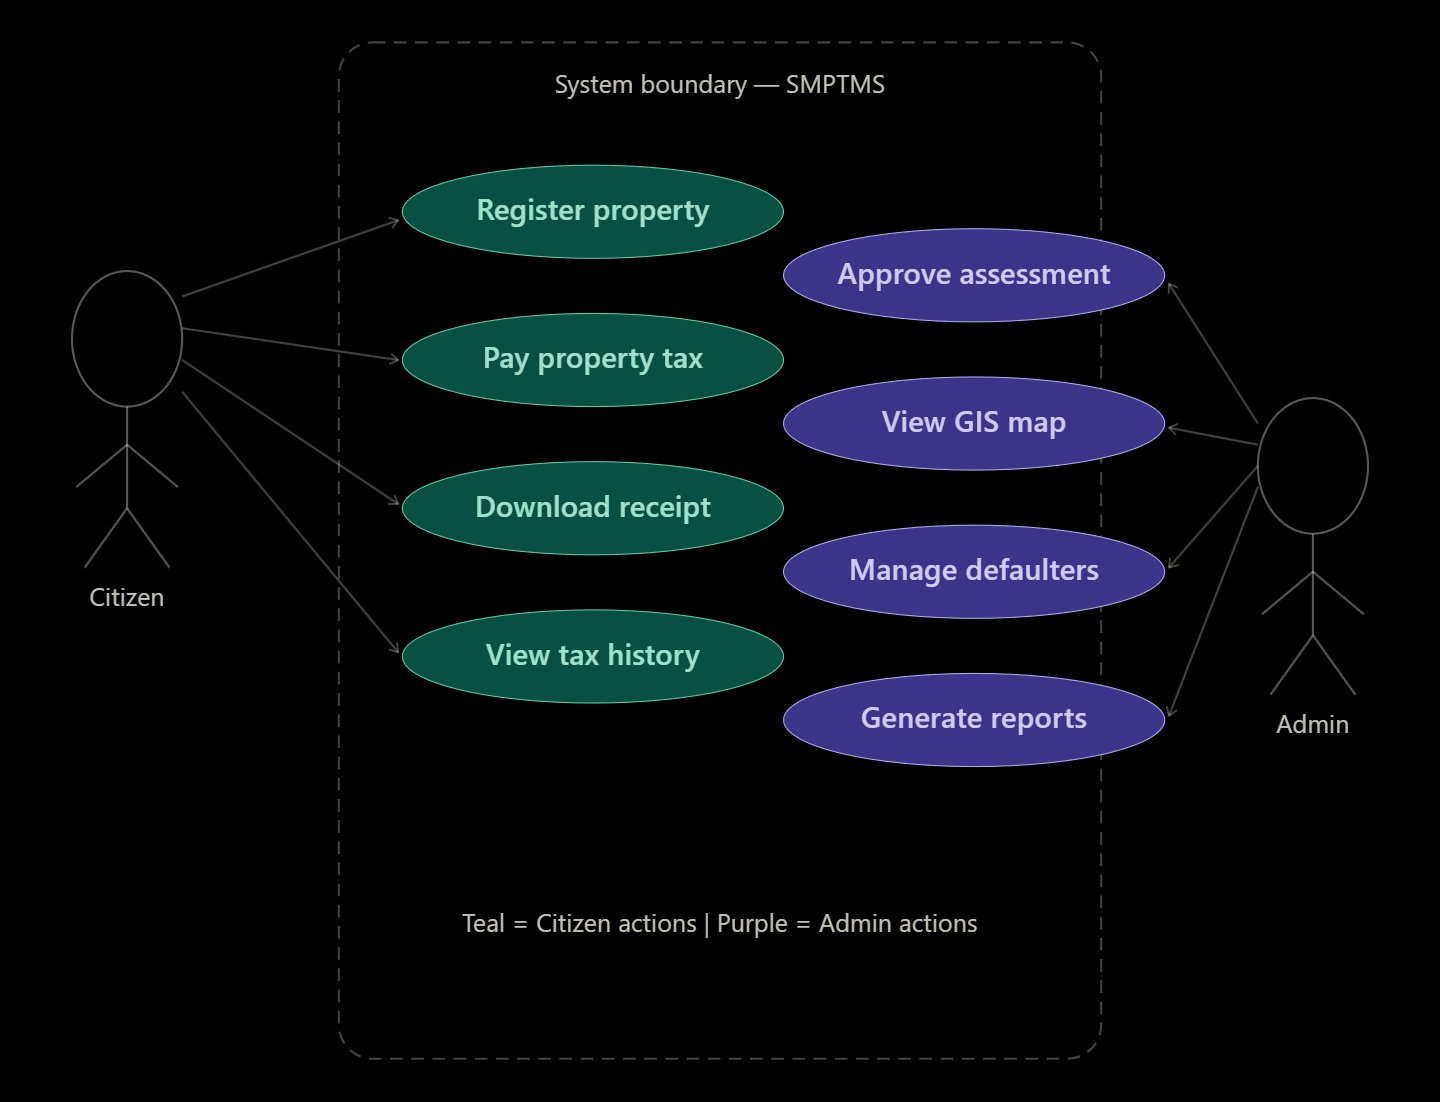
\includegraphics[width=0.85\textwidth]{project/images/usecase.png}\\
  \caption{Use Case Diagram of SMPTMS}
\end{figure}

\subsection{Activity Diagram}
\begin{figure}[H]
  \centering
    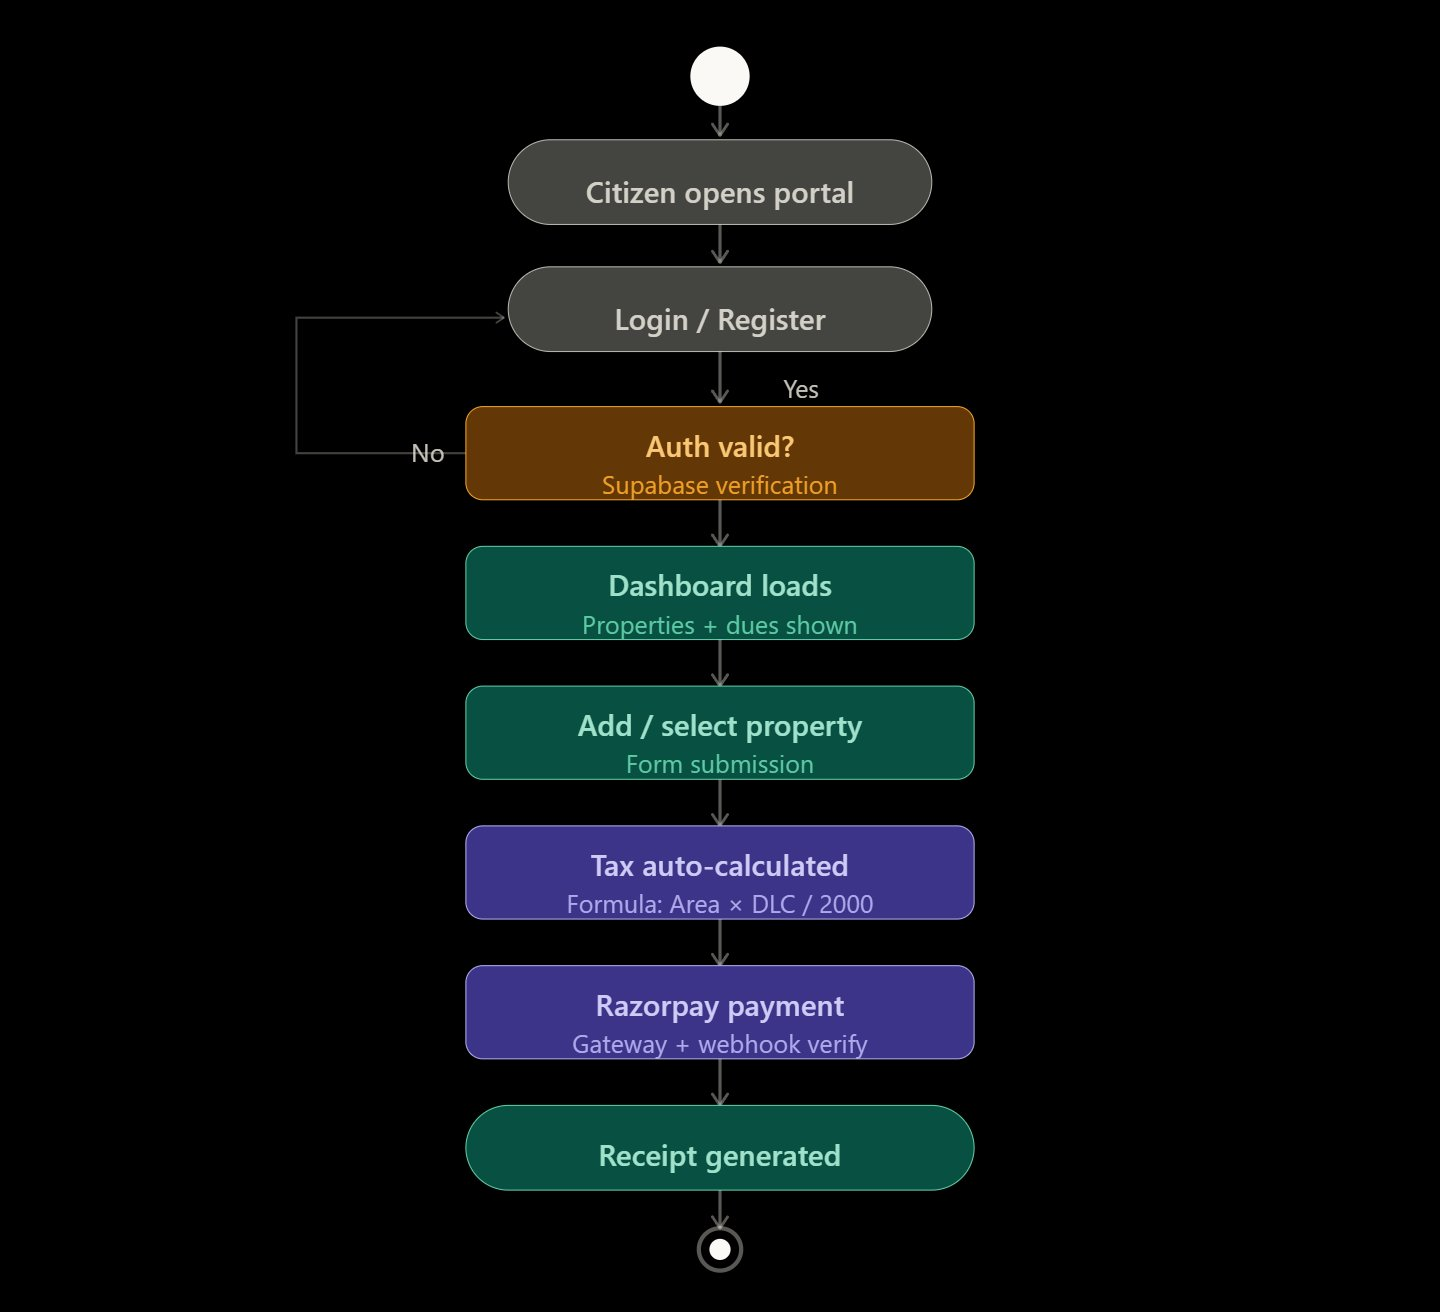
\includegraphics[width=0.75\textwidth]{project/images/activity.png}\\
  \caption{Activity Diagram -- Citizen Tax Payment Flow}
\end{figure}

\subsection{Data-Flow Diagram}
\begin{figure}[H]
  \centering
    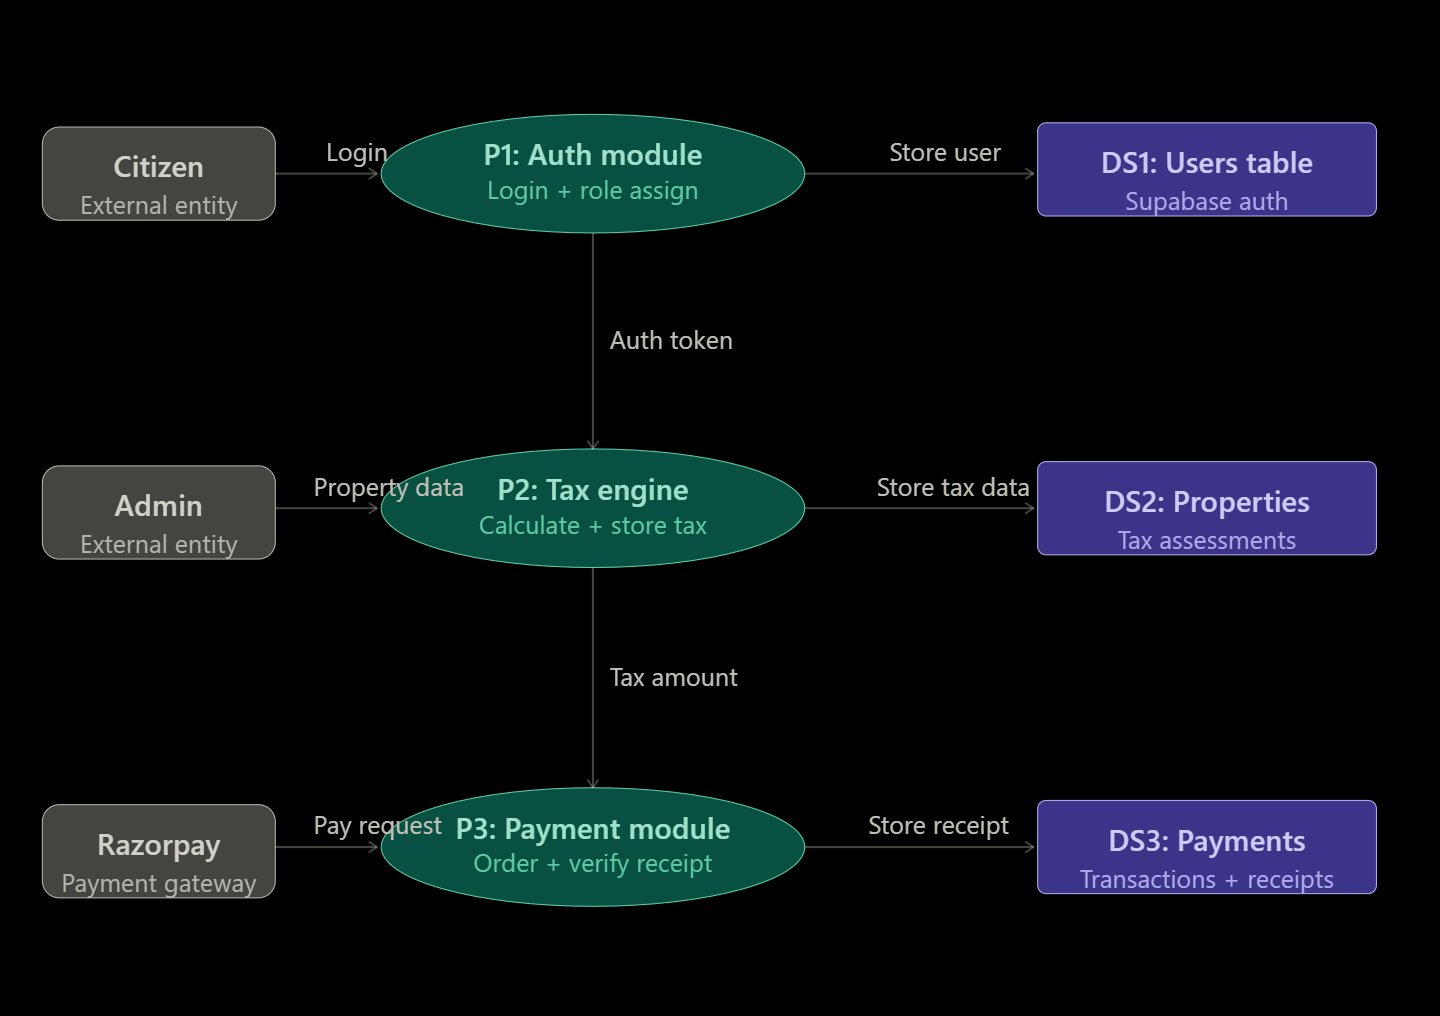
\includegraphics[width=0.85\textwidth]{project/images/data-sync.png}\\
  \caption{Data-Flow Diagram of SMPTMS}
\end{figure}

\subsection{Class Diagram}
\begin{figure}[H]
  \centering
    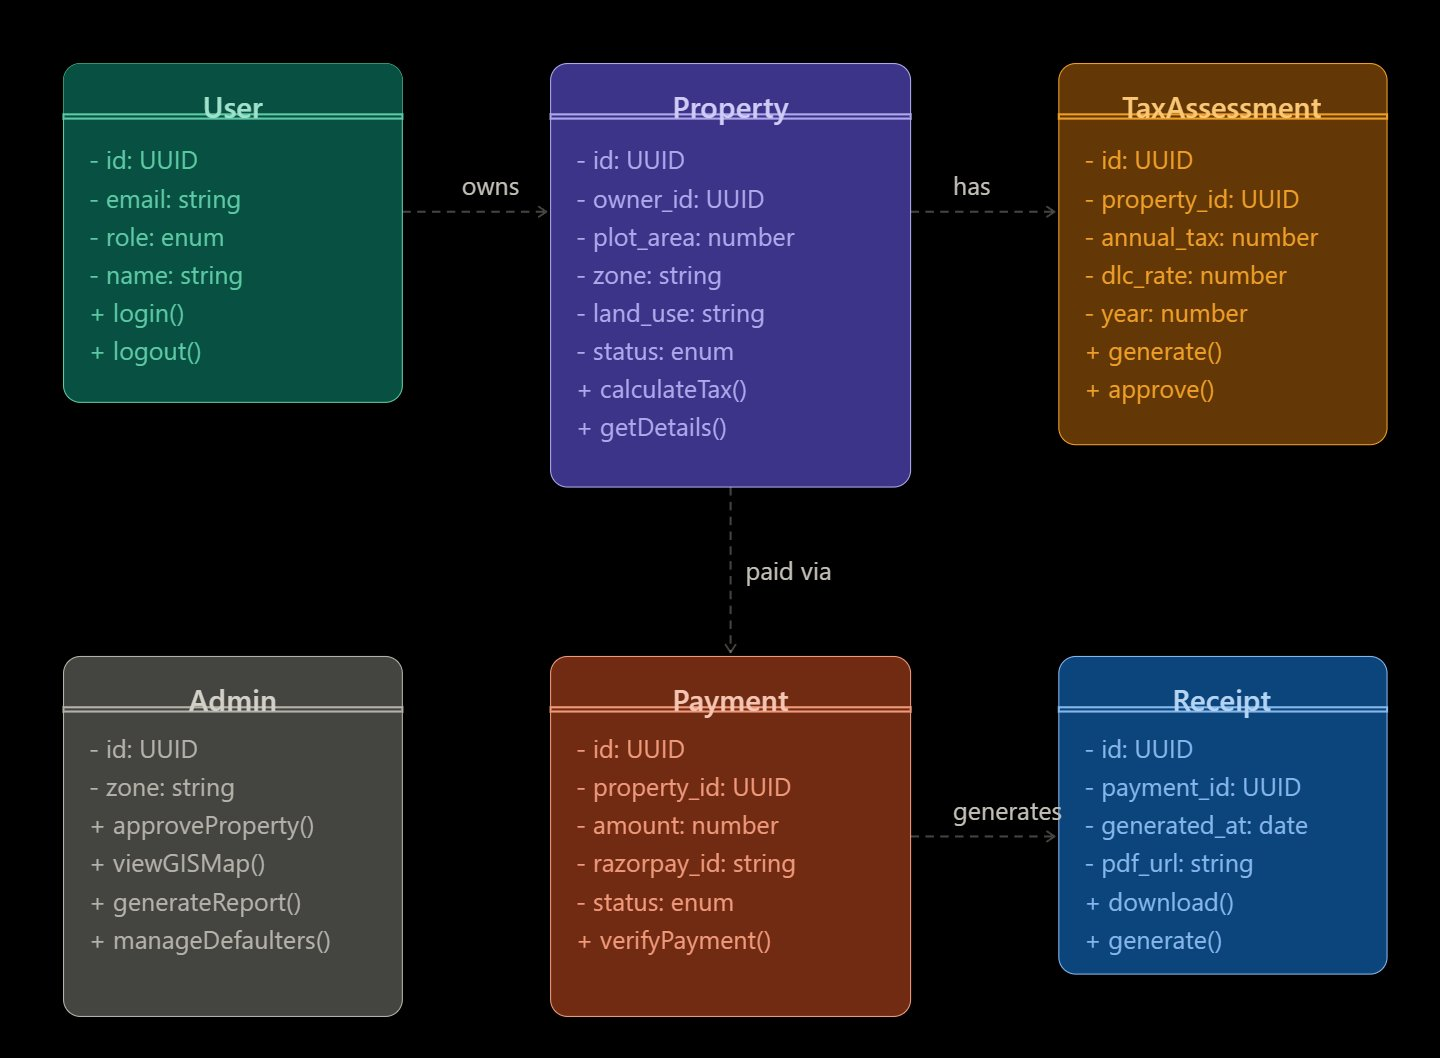
\includegraphics[width=0.85\textwidth]{project/images/classDiagram.png}\\
  \caption{Class Diagram of SMPTMS}
\end{figure}

\subsection{Sequence Diagram}
\begin{figure}[H]
  \centering
    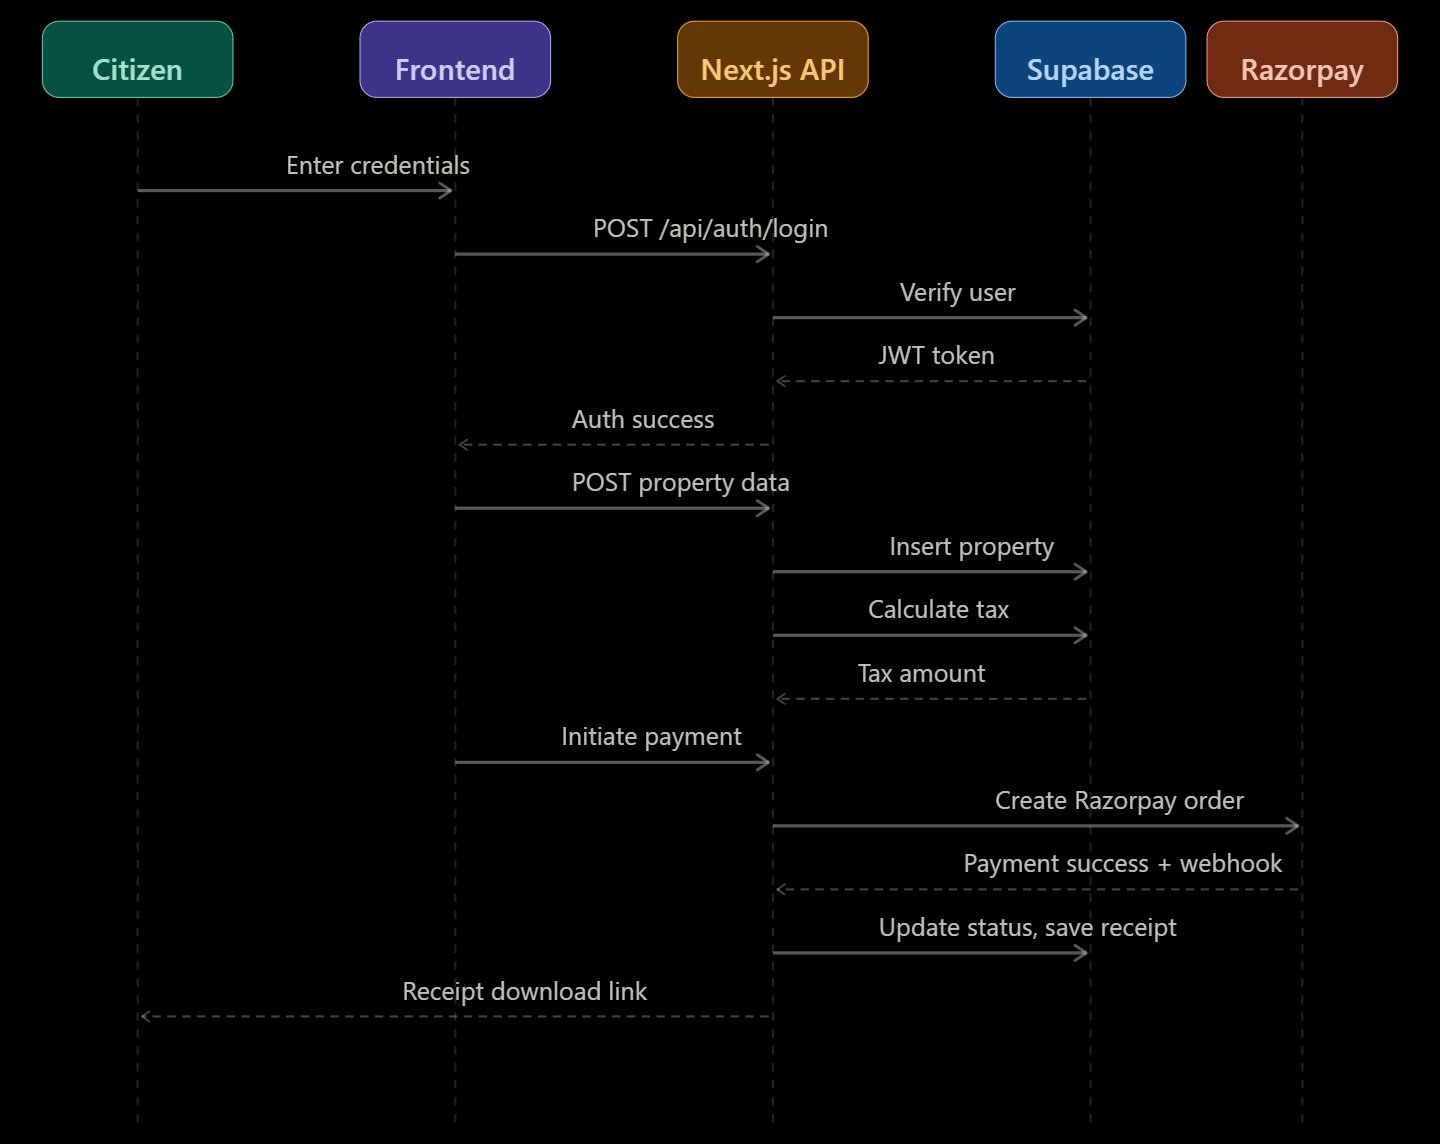
\includegraphics[width=0.85\textwidth]{project/images/seq.png}\\
  \caption{Sequence Diagram -- Payment Processing Flow}
\end{figure}

\chapter{Methodology and Team}
\section{Introduction to Agile Methodology}
\paragraph{}
Agile Methodology is an iterative project management approach that organizes development into short, repeating cycles called sprints. Rather than delivering a complete product at the end of a long development period, Agile teams deliver working increments regularly, allowing for continuous feedback, adaptation, and improvement throughout the project.

For SMPTMS, Agile was adopted because the project involved four modules developed simultaneously by different team members, requiring tight coordination and frequent integration checks. The iterative approach allowed the team to adjust requirements and priorities based on testing outcomes at each sprint boundary.

\paragraph{}The sequential phases in the Agile model as applied to SMPTMS are described below:
\begin{enumerate}
    \item \textbf{Requirement Gathering:} The team conducted an initial analysis of Jaipur Nagar Nigam's property tax pain points, reviewed similar municipal platforms (PCMC Pune, BBMP Bengaluru), and defined the functional and non-functional requirements documented in the SRS. Key requirements such as GIS map integration, Razorpay payment, and role-based access were identified and prioritized in this phase.
    
    \item \textbf{Design:} System architecture, database schema (Supabase PostgreSQL), API route structure (Next.js App Router), and high-level design diagrams (use case, activity, DFD, class, and sequence) were prepared. The three-tier architecture and module decomposition were finalized to enable parallel development across the four team modules.
    
    \item \textbf{Development (Coding):} Each team member developed their assigned module iteratively. Khushal Jangid built the authentication and user dashboard, Gaurav Pratap Singh implemented the tax calculation engine, Kapil Jarwal set up the testing infrastructure and deployment pipeline, and Himanshu Meena developed the GIS mapping and survey features. Weekly syncs ensured module compatibility.
    
    \item \textbf{Testing:} Unit testing, integration testing, and system testing were performed progressively. Postman was the primary API testing tool, supplemented by manual browser testing for UI flows. Test cases for all four modules are documented in Chapter 5.

    \item \textbf{Deployment:} The application was deployed to Vercel's cloud platform with continuous deployment configured from the GitHub repository. Supabase provided the managed PostgreSQL backend and Razorpay was configured with both sandbox (test) and production credentials.

    \item \textbf{Maintenance:} Post-deployment, the team monitored Vercel logs and Supabase query performance to resolve any runtime issues. Bug reports identified during final testing were tracked and resolved before the project report submission deadline.
\end{enumerate}

\section{Team Members, Roles \& Responsibilities}
\begin{table}[H]
\begin{center}
 \begin{tabular}{| m{4cm} | m{2.5cm} | m{2.5cm}| m{5cm}| } 
\hline
\multicolumn{2}{|l|}{MEMBER 1: Khushal Jangid (22ESKCA057)}&
\multicolumn{2}{|l|}{NAME OF MODULE: User Management}\\
\hline
\textbf{NAME OF FUNCTIONALITY} & \textbf{SOFT DEADLINE} & \textbf{HARD DEADLINE} & \textbf{DETAILS OF FUNCTIONALITY} \\ 
\hline
Setup \& Grid & 30/8/25 & 10/9/25 & React.js frontend, Node.js backend setup, login using Next Auth \\
\hline
Styling & 18/8/25 & 25/9/25 & Design UI for user authentication and profile management \\
\hline
Integration (Auth) & 20/9/25 & 10/10/25 & Implement JWT authentication, user dashboard to view profile \\
\hline
User Dashboard & 21/10/25 & 28/11/25 & Create User APIs for registration, login, and data handling \\
\hline
Backend API & 10/11/25 & 28/11/25 & Develop CRUD APIs with tax API and error handling \\
\hline
Tech Integration & 10/12/25 & 30/12/25 & Integrate user details with better UX and error handling \\
\hline
Final Adjustment & 30/1/26 & 20/1/26 & Polish frontend with module testing and documentation \\
\hline
Documentation & 28/2/26 & 20/2/26 & Conduct User Module Testing and Calculation \\
\hline
\end{tabular}
\caption{Member-1 Roles and Responsibilities}
\end{center}
\end{table}

\begin{table}[H]
\begin{center}
 \begin{tabular}{| m{4cm} | m{2.5cm} | m{2.5cm}| m{5cm}| } 
\hline
\multicolumn{2}{|l|}{MEMBER 2: Gaurav Pratap Singh (22ESKCA035)}&
\multicolumn{2}{|l|}{NAME OF MODULE: Tax Calculation}\\
\hline
\textbf{NAME OF FUNCTIONALITY} & \textbf{SOFT DEADLINE} & \textbf{HARD DEADLINE} & \textbf{DETAILS OF FUNCTIONALITY} \\ 
\hline
Schema Design & 28/8/25 & 30/8/25 & Design Supabase schema for tax records, property and income \\
\hline
Tax Data Entry Module & 20/9/25 & 25/9/25 & Create form for property entry and tax function \\
\hline
Tax Logic & 27/10/25 & 30/10/25 & Implement calculation logic: Tax = (Plot Area x DLC Rate) / 2000 \\
\hline
API Development & 25/11/25 & 30/11/25 & Build API routes for entries and data sync \\
\hline
Integration (Supabase) & 15/12/25 & 30/12/25 & Add input validation and tax reports \\
\hline
Error Handling & 10/1/26 & 15/1/26 & Auto-generate tax reports of non-compliant entries \\
\hline
Report Generation & 10/2/26 & 15/2/26 & Integrate tax reports with frontend dashboard \\
\hline
Final Integration & 23/2/26 & 15/3/26 & Final testing of Tax Calculation module \\
\hline
\end{tabular}
\caption{Member-2 Roles and Responsibilities}
\end{center}
\end{table}

\begin{table}[H]
\begin{center}
 \begin{tabular}{| m{4cm} | m{2.5cm} | m{2.5cm}| m{5cm}| } 
\hline
\multicolumn{2}{|l|}{MEMBER 3: Kapil Jarwal (22ESKCA054)}&
\multicolumn{2}{|l|}{NAME OF MODULE: Testing Module}\\
\hline
\textbf{NAME OF FUNCTIONALITY} & \textbf{SOFT DEADLINE} & \textbf{HARD DEADLINE} & \textbf{DETAILS OF FUNCTIONALITY} \\ 
\hline
Test Environment & 28/8/25 & 30/8/25 & Setup Postman and mock environment for API integration \\
\hline
Integration Testing & 20/9/25 & 25/9/25 & Design testing plan for APIs and automated test cases \\
\hline
Unit Testing Scripts & 21/10/25 & 27/10/25 & Create automated test cases for user and tax modules \\
\hline
API Testing & 25/11/25 & 30/12/25 & Testing all backend endpoints and integration points \\
\hline
Bug Report Sheet & 25/11/25 & 15/1/26 & Maintaining test results, deploy system on Vercel \\
\hline
Development Setup & 15/1/26 & 15/2/26 & Final test execution and environment validation \\
\hline
Final Testing & 28/2/26 & 15/3/26 & End-to-end system testing on live deployment \\
\hline
Documentation & -- & -- & Complete documentation of all test cases and results \\
\hline
\end{tabular}
\caption{Member-3 Roles and Responsibilities}
\end{center}
\end{table}

\begin{table}[H]
\begin{center}
 \begin{tabular}{| m{4cm} | m{2.5cm} | m{2.5cm}| m{5cm}| } 
\hline
\multicolumn{2}{|l|}{MEMBER 4: Himanshu Meena (22ESKCA047)}&
\multicolumn{2}{|l|}{NAME OF MODULE: Surveying / GIS}\\
\hline
\textbf{NAME OF FUNCTIONALITY} & \textbf{SOFT DEADLINE} & \textbf{HARD DEADLINE} & \textbf{DETAILS OF FUNCTIONALITY} \\ 
\hline
Land Survey Form & 2/8/25 & 12/8/25 & Survey form: Parcel ID, area, coordinates \\
\hline
Map Integration & 13/8/25 & 11/9/25 & Map integration with polygon boundary and document upload \\
\hline
Survey Data Upload & 1/9/25 & 10/10/25 & Document upload, version history, timeline of survey changes \\
\hline
Survey History Tracking & 1/10/25 & 15/11/25 & Admin dashboard for surveyed vs pending properties \\
\hline
Parcel Status Dashboard & 2/11/25 & 12/12/25 & Duplicate parcel detection and geo-conflict handling \\
\hline
Duplicate Parcel Detection & 1/1/26 & 10/1/26 & PDF reports with ward/zone-wise date filters \\
\hline
Survey Report Generation & 1/2/26 & 11/2/26 & Auto alerts via email/SMS on survey updates \\
\hline
Final Integration & 20/2/26 & 15/3/26 & Final GIS module testing and documentation \\
\hline
\end{tabular}
\caption{Member-4 Roles and Responsibilities}
\end{center}
\end{table}

\chapter{System Testing}
\section{Introduction}
\paragraph{}Software testing is the systematic process of evaluating a system to verify that it behaves correctly and meets its specified requirements. For SMPTMS, testing was conducted across three levels --- unit, integration, and full system --- to validate every component before the platform was made available for live use. The primary testing tool was Postman for API-level testing, supplemented by manual browser-based testing for UI workflows and Razorpay's sandbox environment for payment validation.

\section{Types of Testing Performed}
\subsection{Unit Testing}
\paragraph{}Each module was tested independently before integration. The tax calculation engine was tested by running a range of input combinations --- varying plot sizes, zone categories, and DLC rates --- through the formula and verifying computed outputs against manual calculations. The authentication module was tested by attempting valid and invalid login credentials, checking session expiry behaviour, and validating role switching between citizen and admin accounts. Each API endpoint was tested in isolation using Postman to confirm correct status codes, response payloads, and error handling.

\subsection{Integration Testing}
\paragraph{}Integration testing focused on verifying correct data flow between modules. Key integration test scenarios included confirming that a property registered by a citizen appeared immediately on the admin GIS map with the correct zone and status, verifying that a completed Razorpay payment updated the property record in Supabase in real time via the webhook, and ensuring that the receipt generation function correctly pulled transaction details from the payment record. Cross-module interactions between the user management, tax calculation, and payment modules were validated in this phase.

\subsection{System Testing}
\paragraph{}Full end-to-end testing was performed on the live Vercel deployment. Test scenarios covered the complete citizen workflow: account registration, property submission, tax calculation review, Razorpay sandbox payment completion, and receipt download. Admin workflows were also tested: logging in to the admin panel, viewing the GIS property map, filtering by zone and payment status, accessing the defaulter list, and generating zone-wise reports. All tests were repeated after bug fixes to confirm resolution.

\section{Test Cases}
\begin{table}[H]
\begin{center}
 \begin{tabular}{| m{1.2cm} | m{3.5cm} | m{2.2cm}| m{3cm}|m{3cm}| } 
\hline
\multicolumn{3}{|l|}{NAME OF MODULE: User Management}&
\multicolumn{2}{|l|}{TESTING TOOL: Postman + Manual Browser}\\[0.8cm]
\hline
\textbf{Test ID} & \textbf{Test Description} & \textbf{Input Data} & \textbf{Expected Output} & \textbf{Actual Output} \\ 
\hline
TC-UM-01 & Valid user registration & Name: Kapil Jarwal, Email: kapil@gmail.com, Pass: Test@123 & Account created, redirect to dashboard & Account created successfully \\
\hline
TC-UM-02 & Login with correct credentials & Email: kapil@gmail.com, Pass: Test@123 & Dashboard loads with user data & Dashboard loaded correctly \\
\hline
TC-UM-03 & Login with wrong password & Email: kapil@gmail.com, Pass: wrong123 & Error -- Invalid credentials & Error displayed correctly \\
\hline
TC-UM-04 & Login with unregistered email & Email: fake@test.com, Pass: Test@123 & Error -- User not found & Error displayed correctly \\
\hline
TC-UM-05 & Access dashboard without login & Direct URL: /dashboard & Redirected to /login & Redirected correctly \\
\hline
TC-UM-06 & Admin login with citizen credentials & Citizen credentials on admin panel & Access denied, role mismatch & Access correctly blocked \\
\hline
TC-UM-07 & Session timeout check & User idle for extended period & Auto logout, redirect to login & Session expired correctly \\
\hline
TC-UM-08 & Duplicate email registration & Same email registered twice & Error -- Email already exists & Duplicate blocked correctly \\
\hline
\end{tabular}
\caption{Test Cases -- User Management Module}
\end{center}
\end{table}

\begin{table}[H]
\begin{center}
 \begin{tabular}{| m{1.2cm} | m{3.5cm} | m{2.2cm}| m{3cm}|m{3cm}| } 
\hline
\multicolumn{3}{|l|}{NAME OF MODULE: Tax Calculation}&
\multicolumn{2}{|l|}{TESTING TOOL: Postman + Manual Verification}\\[0.8cm]
\hline
\textbf{Test ID} & \textbf{Test Description} & \textbf{Input Data} & \textbf{Expected Output} & \textbf{Actual Output} \\ 
\hline
TC-TC-01 & Basic tax calculation -- Zone C residential & Area: 280 sq.m, Zone C, Residential & Tax = (280 x DLC Rate) / 2000 & Correct amount calculated \\
\hline
TC-TC-02 & Tax calculation -- Zone A commercial & Area: 520 sq.m, Zone A, Commercial & Higher tax due to Zone A DLC rate & Correct amount calculated \\
\hline
TC-TC-03 & Minimum plot size & Area: 50 sq.m, Zone B, Residential & Low tax as per formula & Calculated correctly \\
\hline
TC-TC-04 & Large commercial plot & Area: 2000 sq.m, Zone A, Commercial & Large tax verified manually & Matched manual calculation \\
\hline
TC-TC-05 & Zero area input validation & Area: 0, Zone C & Error -- Invalid plot area & Validation error shown \\
\hline
TC-TC-06 & Negative area input & Area: -100 & Error -- Area cannot be negative & Validation blocked input \\
\hline
TC-TC-07 & DLC rate change effect & Admin updates Zone B DLC rate & New rate applied to Zone B properties & Rate updated correctly \\
\hline
TC-TC-08 & Multiple properties total dues & 2 properties in dashboard & Correct total dues displayed & Correct total displayed \\
\hline
\end{tabular}
\caption{Test Cases -- Tax Calculation Module}
\end{center}
\end{table}

\begin{table}[H]
\begin{center}
 \begin{tabular}{| m{1.2cm} | m{3.5cm} | m{2.2cm}| m{3cm}|m{3cm}| } 
\hline
\multicolumn{3}{|l|}{NAME OF MODULE: Payment and Receipt}&
\multicolumn{2}{|l|}{TESTING TOOL: Postman + Razorpay Sandbox}\\[0.8cm]
\hline
\textbf{Test ID} & \textbf{Test Description} & \textbf{Input Data} & \textbf{Expected Output} & \textbf{Actual Output} \\ 
\hline
TC-PM-01 & Successful payment -- test mode & Razorpay test card, Amount: Rs.1434 & Payment success, status updated to Paid & Payment processed correctly \\
\hline
TC-PM-02 & Payment cancelled by user & User cancels Razorpay popup midway & Payment status remains Pending & Status unchanged correctly \\
\hline
TC-PM-03 & Invalid card details & Card: 0000 0000 0000 0000 & Payment failed, Razorpay error & Failure handled correctly \\
\hline
TC-PM-04 & Receipt generation after payment & Completed payment transaction ID & Downloadable PDF receipt generated & Receipt generated correctly \\
\hline
TC-PM-05 & Payment webhook verification & Razorpay sends signed callback & Backend verifies signature, updates DB & Signature verified correctly \\
\hline
TC-PM-06 & Double payment attempt & Pay again on already-paid property & Warning -- Tax already paid & Blocked correctly \\
\hline
TC-PM-07 & Receipt data accuracy & Download receipt after payment & Correct name, amount, date, property & All fields matched correctly \\
\hline
TC-PM-08 & Admin real-time status update & Payment completed by citizen & Admin panel reflects paid status instantly & Real-time update confirmed \\
\hline
\end{tabular}
\caption{Test Cases -- Payment and Receipt Module}
\end{center}
\end{table}

\begin{table}[H]
\begin{center}
 \begin{tabular}{| m{1.2cm} | m{3.5cm} | m{2.2cm}| m{3cm}|m{3cm}| } 
\hline
\multicolumn{3}{|l|}{NAME OF MODULE: Surveying / GIS Map}&
\multicolumn{2}{|l|}{TESTING TOOL: Manual Browser + Leaflet.js Inspector}\\[0.8cm]
\hline
\textbf{Test ID} & \textbf{Test Description} & \textbf{Input Data} & \textbf{Expected Output} & \textbf{Actual Output} \\ 
\hline
TC-GIS-01 & Map loads with Jaipur coordinates & Open /dashboard/map & Map centred on Jaipur, all markers visible & Map loaded correctly \\
\hline
TC-GIS-02 & Paid property marker colour & Property with paid status & Green marker on map & Green marker displayed \\
\hline
TC-GIS-03 & Pending property marker colour & Property with pending status & Orange marker on map & Orange marker displayed \\
\hline
TC-GIS-04 & Search by property owner name & Search: Rajesh Kumar & Sidebar highlights property, map pans to location & Search worked correctly \\
\hline
TC-GIS-05 & Filter pending properties only & Click Pending filter & Only pending properties shown & Filter applied correctly \\
\hline
TC-GIS-06 & Filter paid properties only & Click Paid filter & Only paid properties shown & Filter applied correctly \\
\hline
TC-GIS-07 & Property popup on marker click & Click any map marker & Popup shows owner, zone, tax, status & Popup displayed correctly \\
\hline
TC-GIS-08 & Satellite view toggle & Click Satellite button & Map tiles switch to satellite imagery & Toggle worked correctly \\
\hline
TC-GIS-09 & Total property count accuracy & 21 properties in database & Header shows 21 Total & Count matched correctly \\
\hline
TC-GIS-10 & Map responsive on mobile & Open map on mobile browser & Map renders correctly, controls accessible & Responsive confirmed \\
\hline
\end{tabular}
\caption{Test Cases -- GIS Map and Surveying Module}
\end{center}
\end{table}

\chapter{Project Screenshots}
\section{Introduction}
\paragraph{}This chapter presents screenshots of the SMPTMS platform captured from the live deployment at smptms.vercel.app. The screenshots illustrate key interfaces including the citizen login page, citizen dashboard, property registration form, tax calculation result, Razorpay payment gateway, receipt download screen, admin panel overview, and the GIS property map. These visuals demonstrate the system's functionality and user experience as delivered in the final deployed version.

\section{Citizen Interface}
\paragraph{}The citizen-facing interface provides a clean, guided experience for property owners to manage their tax obligations. Below are the key screens from the citizen workflow.

\begin{figure}[H]
  \centering
  \fbox{\rule{0pt}{8cm}\rule{12cm}{0pt}}
  \caption{Login / Registration Page -- Citizen Portal}
\end{figure}

\begin{figure}[H]
  \centering
  \fbox{\rule{0pt}{8cm}\rule{12cm}{0pt}}
  \caption{Citizen Dashboard -- Property Portfolio and Dues Overview}
\end{figure}

\begin{figure}[H]
  \centering
  \fbox{\rule{0pt}{8cm}\rule{12cm}{0pt}}
  \caption{Add Property Form -- Plot Details and Zone Selection}
\end{figure}

\begin{figure}[H]
  \centering
  \fbox{\rule{0pt}{8cm}\rule{12cm}{0pt}}
  \caption{Tax Calculation Result -- Computed Annual Tax Display}
\end{figure}

\begin{figure}[H]
  \centering
  \fbox{\rule{0pt}{8cm}\rule{12cm}{0pt}}
  \caption{Razorpay Payment Gateway -- Checkout Screen}
\end{figure}

\begin{figure}[H]
  \centering
  \fbox{\rule{0pt}{8cm}\rule{12cm}{0pt}}
  \caption{Payment Success Confirmation and Receipt Download}
\end{figure}

\section{Admin Interface}
\paragraph{}The administrative panel provides municipal officials with complete visibility into the property tax system across all registered properties and zones in Jaipur.

\begin{figure}[H]
  \centering
  \fbox{\rule{0pt}{8cm}\rule{12cm}{0pt}}
  \caption{Admin Dashboard -- System Overview and Statistics}
\end{figure}

\begin{figure}[H]
  \centering
  \fbox{\rule{0pt}{8cm}\rule{12cm}{0pt}}
  \caption{GIS Property Map -- Jaipur with Colour-Coded Payment Status Markers}
\end{figure}

\begin{figure}[H]
  \centering
  \fbox{\rule{0pt}{8cm}\rule{12cm}{0pt}}
  \caption{Defaulter Tracking List -- Pending Properties by Zone}
\end{figure}

\begin{figure}[H]
  \centering
  \fbox{\rule{0pt}{8cm}\rule{12cm}{0pt}}
  \caption{Zone-wise Tax Collection Report}
\end{figure}

\paragraph{}\textit{Note: The placeholder boxes above represent screenshot locations. Replace each box with the corresponding application screenshot before final binding. Screenshots can be added using the LaTeX command: \textbackslash includegraphics[width=0.9\textbackslash textwidth]\{project/images/screenshot-name.png\}}

\chapter{Conclusion and Future Scope}
\section{Conclusion}
\paragraph{}The Smart Property Tax Management System (SMPTMS) demonstrates that a fully functional, transparent, and efficient property tax platform does not require expensive infrastructure or complex technical operations. By combining Next.js 14, Supabase, Leaflet.js, and Razorpay into a cohesive, well-architected system, the project delivers a practical solution to a problem that affects municipal revenue collection across hundreds of Indian cities.

\paragraph{}The platform successfully digitizes the complete property tax lifecycle for Jaipur Nagar Nigam. Citizens can register properties and complete tax payments in under three minutes from any device with a browser. The tax calculation formula is fixed, publicly visible, and applied uniformly across all zones, eliminating the scope for manual manipulation that has historically eroded public trust in municipal assessment processes.

\paragraph{}Administrators gain real-time visibility into the city's tax compliance picture through the GIS-based property map, enabling data-driven decisions about enforcement and revenue planning. The system is live, tested across all four modules, and operational at smptms.vercel.app. The project achieves its primary objective: removing the friction points of confusion, inaccessibility, and distrust that have historically suppressed property tax compliance in smaller Indian cities.

\section{Future Scope}
\paragraph{}Several meaningful extensions to SMPTMS have been identified for future development:
\begin{itemize}
 \item Integration with Rajasthan's state-level ULBHRMS platform to enable automatic data synchronization across all municipalities in the state, reducing duplication of records and enabling unified statewide revenue reporting.
 \item Development of a dedicated mobile application for iOS and Android with push notification reminders for upcoming dues, payment history access, and offline property detail viewing.
 \item Implementation of AI-based property anomaly detection using satellite imagery analysis to identify potentially undervalued or unregistered properties in Jaipur's developing zones.
 \item Multi-language support including Hindi and Rajasthani dialects to improve accessibility for less digitally literate property owners in rural wards.
 \item WhatsApp Business API integration to deliver automated payment reminders and official tax receipt PDFs directly to citizens' WhatsApp numbers, reducing the barrier to receipt access.
 \item Extension of the platform to cover additional municipal revenue streams such as trade licenses, water bills, and building plan approval fees within the same unified portal.
\end{itemize}

\chapter{UN Sustainable Development Goals}
\section{Mapping with UN Sustainable Development Goals}
\paragraph{}The 2030 Agenda for Sustainable Development, adopted by 193 Member States at the UN General Assembly Summit in September 2015, defines 17 Sustainable Development Goals (SDGs) covering economic, social, and environmental dimensions of global development. Every project undertaken in academic and professional contexts should be evaluated for its contribution toward one or more of these goals.

\paragraph{}SMPTMS --- Smart Property Tax Management System --- directly aligns with \textbf{SDG 11: Sustainable Cities and Communities}, which aims to make cities inclusive, safe, resilient, and sustainable. A key enabler of sustainable urban governance is the financial independence of municipalities. Property tax is the most significant own-source revenue stream for Urban Local Bodies in India. By digitizing and streamlining property tax collection for Jaipur Nagar Nigam, SMPTMS contributes to stronger municipal finances, more transparent governance, and improved delivery of urban services for all citizens.

\begin{table}[h]
    \begin{tabular}{|l|p{6cm}|p{8cm}|}
        \hline
        \multicolumn{3}{|l|}{\textbf{SDG Title: SDG 11 -- Sustainable Cities and Communities}} \\
        \hline
        \textbf{S.No} & \textbf{Objective} & \textbf{Outcome} \\
        \hline
        1 & Improve municipal revenue collection through digitization of property tax administration & Increased tax compliance leading to better funding for civic infrastructure including roads, sanitation, and water supply in Jaipur \\
        \hline
        2 & Make property tax assessment transparent and accessible to all citizens regardless of digital literacy level & Reduced scope for corruption and manual manipulation in tax calculations through a publicly visible, formula-based system \\
        \hline
        3 & Enable online payment to remove physical barriers for citizens in remote wards who cannot easily visit municipal offices & Higher payment rates and reduced administrative burden on ward-level staff, enabling faster revenue realization \\
        \hline
        4 & Provide GIS-based property mapping to support evidence-based urban planning and property record maintenance & Accurate, spatially-referenced property data enabling smarter infrastructure investment decisions by Jaipur Nagar Nigam \\
        \hline
    \end{tabular}
    \caption{SDG 11 Mapping for SMPTMS}
    \label{tab:sdg}
\end{table}

\addcontentsline{toc}{chapter}{References}
\begin{thebibliography}{99}

\bibitem{ref1}
I. Sommerville,
\textit{Software Engineering},
10th ed. Boston, MA, USA: Pearson, 2016.

\bibitem{ref2}
R. S. Pressman and B. R. Maxim,
\textit{Software Engineering: A Practitioner's Approach},
8th ed. New York, NY, USA: McGraw-Hill Education, 2014.

\bibitem{ref3}
Ministry of Housing and Urban Affairs, Government of India,
``Municipal Finances in India: A Study of Property Tax,''
\textit{National Institute of Urban Affairs Report},
New Delhi, India, 2021.

\bibitem{ref4}
S. Rajasekaran and G. A. Vijayalakshmi Pai,
\textit{Neural Networks, Fuzzy Logic, and Genetic Algorithms: Synthesis and Applications},
New Delhi, India: Prentice-Hall of India, 2010.

\bibitem{ref5}
Next.js Documentation,
``App Router -- Introduction,''
Vercel Inc., 2024. [Online].
Available: https://nextjs.org/docs

\bibitem{ref6}
Supabase Documentation,
``Supabase Auth and PostgreSQL,''
Supabase Inc., 2024. [Online].
Available: https://supabase.com/docs

\bibitem{ref7}
Razorpay,
``Razorpay Payment Integration Guide,''
Razorpay Software Pvt. Ltd., 2024. [Online].
Available: https://razorpay.com/docs

\bibitem{ref8}
Leaflet.js Documentation,
``Leaflet -- an open-source JavaScript library for mobile-friendly interactive maps,''
2024. [Online].
Available: https://leafletjs.com/reference.html

\bibitem{ref9}
Government of Rajasthan,
``District Level Circle (DLC) Rates -- Jaipur District,''
Stamps and Registration Department, Rajasthan, 2024.

\bibitem{ref10}
Ministry of Housing and Urban Affairs,
``Smart Cities Mission -- Digital Urban Governance Framework,''
Government of India, New Delhi, 2022.

\bibitem{ref11}
P. Ghosh and P. Bandyopadhyay,
``Digitization of Property Tax in Urban Local Bodies: Evidence from Indian Cities,''
\textit{Journal of Urban Economics and Management},
vol. 8, no. 2, pp. 45--62, 2022.

\bibitem{ref12}
T. H. Cormen, C. E. Leiserson, R. L. Rivest, and C. Stein,
\textit{Introduction to Algorithms},
3rd ed. Cambridge, MA, USA: MIT Press, 2009.

\end{thebibliography}

\chapter*{Project Poster}
\addcontentsline{toc}{chapter}{Project Poster}
\paragraph{}\textit{(Attach your project poster here. The poster should cover the project title, problem statement, proposed solution, tech stack, key features, system architecture diagram, and team members. Recommended size: A1 or A2 format.)}

\begin{figure}[H]
  \centering
  \fbox{\rule{0pt}{16cm}\rule{12cm}{0pt}}
  \caption{SMPTMS Project Poster -- Smart Property Tax Management System}
\end{figure}

\chapter*{Certificate of Achievement}
\addcontentsline{toc}{chapter}{Certificate}
\paragraph{}This section should contain certificates as proof of participation in any of the following activities undertaken by team members during the project period:

\begin{itemize}
    \item Hackathon participation or winning certificate
    \item Research paper publication, presentation, or acceptance email
    \item Poster competition participation or award certificate
    \item Patent filing acknowledgement
\end{itemize}

\paragraph{}\textit{(Attach relevant certificates here before final binding. If your research paper has been accepted but not yet published, include a screenshot of the acceptance email from the conference or journal.)}

\chapter*{Plagiarism Report}
\addcontentsline{toc}{chapter}{Plagiarism Report}
\paragraph{}Attach the plagiarism/similarity report here as proof that the overall similarity index is below 20\% and no single source exceeds 5\%. The report must show 0\% AI-generated content.
\paragraph{}\textit{(Paste or attach your Turnitin / iThenticate / Unicheck similarity report screenshot or PDF here before final binding.)}

\chapter*{GitHub Link}
\addcontentsline{toc}{chapter}{GitHub Link}
\section*{Project Repository:}
\large{\textbf{GitHub:} \url{https://github.com/kapilk8/smptms}}

\section*{Live Deployment:}
\large{\textbf{Vercel:} \url{https://smptms.vercel.app}}

\section*{Project Details:}
\begin{table}[H]
\begin{center}
\begin{tabular}{| m{5cm} | m{9cm} |}
\hline
\textbf{Project Name} & Smart Property Tax Management System (SMPTMS) \\
\hline
\textbf{Project ID} & SKIT/2025-26/AI/Group-03 \\
\hline
\textbf{Tech Stack} & Next.js 14, TypeScript, Supabase, Tailwind CSS, Leaflet.js, Razorpay \\
\hline
\textbf{Deployment Platform} & Vercel \\
\hline
\textbf{Database} & Supabase (PostgreSQL) \\
\hline
\textbf{Payment Gateway} & Razorpay \\
\hline
\textbf{Session} & 2025 -- 2026 \\
\hline
\end{tabular}
\caption{Project Technical Summary}
\end{center}
\end{table}


\end{document}
